\section{Distances to the discrete measure implied by RH}\label{ch:distances}



On a window where the zeros are known, the Thorin measure $\mu_\varepsilon$ computed by the P\'olya route can be compared with $U_{\RH}$ directly (Section~\ref{sec:ch6:measure}), and how close the two are depends on the metric.

Fix $\Theta=200$ and the window $E=(0,\Theta^2]$ in $z$, equivalently $(0,\Theta]$ in $\theta$. The window contains $79$ zeros, all simple and on the line, and $\Theta$ is not an ordinate, since $\gamma_{80}=201.2648$ (Section~\ref{sec:ch4:height200}). For a signed measure $\nu$ on $E$ write $\tv{\nu}=|\nu|(E)$, and write $M_\varepsilon(\theta)=\mu_\varepsilon((0,\theta^2])$ for the cumulative mass.

\subsection{Total variation at matched resolution}\label{sec:ch7:matched}

A smooth approximation to a sum of point masses never converges to it in total variation.

\begin{proposition}\label{prop:raw}
If $\nu\ge0$ is absolutely continuous and $U$ is purely atomic with $N$ unit atoms in $E$, then $\tv{\nu-U}=\nu(E)+N$.
\end{proposition}

\begin{proof}
Let $A$ be the finite set of atoms. Then $\nu(A)=0$, so $|\nu-U|(A)=U(A)=N$ and $|\nu-U|(E\setminus A)=\nu(E\setminus A)=\nu(E)$.
\end{proof}

The Thorin measure is positive on $E$, where its density has minimum $0.0147\,\varepsilon$ (Section~\ref{sec:ch6:measure}), so $\tv{\mu_\varepsilon-U_{\RH}}=\mu_\varepsilon(E)+79\approx158$ for every $\varepsilon$. Total variation becomes informative only after both measures have been brought to the same resolution, or summed over cells.

By Proposition~\ref{prop:struct} the object to compare with $\mu_\varepsilon$ is the Poisson smoothing of the RH measure at the same resolution, and we write $d_{\rm match}(\varepsilon)=\tv{\mu_\varepsilon-P_\varepsilon*U^\pm_{\RH}}$ for the matched distance. Under RH the two measures coincide and $d_{\rm match}(\varepsilon)=0$, so a computation of the matched distance measures its own error unless some zero is off the line.

A computation replaces $U^\pm_{\RH}$ by a model $\widetilde U$, which we build from the first $1700$ ordinates, computed with \texttt{mpmath} \cite{mpmath}, and from the smooth density $\pi^{-1}\vartheta'(t)\,dt$ of the Riemann Siegel theta function beyond the Gram point $T_*=g_{1699}=2197.8796$ of Section~\ref{sec:ch5:turing}, at which $\vartheta(T_*)/\pi+1=1700$, each with its reflection. We write $\tilde d_{\rm match}(\varepsilon)=\tv{\mu_\varepsilon-P_\varepsilon*\widetilde U}$ for the matched distance against the model. Since $\gamma_{1700}=2197.2587<T_*<\gamma_{1701}=2198.6875$, we have $N(T_*)=\vartheta(T_*)/\pi+1$, so the boundary term vanishes when $\int_{T_*}^\infty P_\varepsilon(\theta-t)\,d\big(N(t)-\vartheta(t)/\pi-1\big)$ is integrated by parts, and the error of the tail model is at most of order $\varepsilon/T_*^2$ per unit length. The observed floor is far smaller: $\tilde d_{\rm match}(\varepsilon)=3.66\times10^{-9}\,\varepsilon$ at every resolution from $\varepsilon=1$ to $\varepsilon=0.005$ (Table~\ref{tab:tv}), that is $1.8\times10^{-11}\,\varepsilon$ per unit length. The exact proportionality to $\varepsilon$ identifies the floor as the residual of the tail model; it is an observed value, not a bound for $d_{\rm match}(\varepsilon)$: such a bound would need certified bounds on the error of the tail model and on the evaluation of $\mu_\varepsilon$. The densities that enter the comparison are stored in double precision.

\begin{table}[t]
\centering\small\setlength{\tabcolsep}{4pt}
\begin{tabular}{rrrrrrrr}
\toprule
$\varepsilon$ & mass & raw TV & matched TV & sup diff & cell TV & $L^1$ in $\theta$ & $W_\varepsilon(0.01)$\\
\midrule
1 & 79.36738 & 158.37 & $3.66\times10^{-9}$ & $1.9\times10^{-11}$ & 4.992 & 59.23 & 0.29504\\
0.5 & 79.19417 & 158.19 & $1.83\times10^{-9}$ & $9.6\times10^{-12}$ & 2.655 & 41.86 & 0.22362\\
0.25 & 79.09887 & 158.10 & $9.14\times10^{-10}$ & $4.8\times10^{-12}$ & 1.351 & 28.77 & 0.18698\\
0.1 & 79.03977 & 158.04 & $3.66\times10^{-10}$ & $1.9\times10^{-12}$ & 0.5431 & 16.01 & 0.16469\\
0.05 & 79.01990 & 158.02 & $1.83\times10^{-10}$ & $9.6\times10^{-13}$ & 0.2718 & 9.737 & 0.15721\\
0.02 & 79.00796 & 158.01 & $7.31\times10^{-11}$ & $3.8\times10^{-13}$ & 0.1087 & 4.816 & 0.15270\\
0.01 & 79.00398 & 158.00 & $3.66\times10^{-11}$ & $2.0\times10^{-13}$ & 0.05437 & 2.756 & 0.15120\\
0.005 & 79.00199 & 158.00 & $1.83\times10^{-11}$ & $1.5\times10^{-13}$ & 0.02718 & 1.553 & 0.15045\\
\midrule
RH & 79 & 0 & 0 & 0 & 0 & 0 & 0.14970\\
\bottomrule
\end{tabular}
\caption{Distances between the P\'olya computed Thorin measure $\mu_\varepsilon$ and $U_{\RH}$ on $0<z\le200^2$. Mass is $M_\varepsilon(200)$. Raw TV is $\tv{\mu_\varepsilon-U_{\RH}}$, forced to equal mass plus $79$ by Proposition~\ref{prop:raw}. Matched TV is $\tilde d_{\rm match}(\varepsilon)=\tv{\mu_\varepsilon-P_\varepsilon*\widetilde U}$, and sup diff is the maximum of $|\rho_\varepsilon-P_\varepsilon*\widetilde U|$ over $0<\theta\le200$. Cell TV is $d_{\rm cell}(\varepsilon)$, $L^1$ in $\theta$ is $\int_0^{200}|M_\varepsilon-N|\,d\theta$, and $W_\varepsilon(0.01)$ is the smoothed heat trace at $t=0.01$, with the value from the zeros in the last row.}
\label{tab:tv}
\end{table}

\subsection{Cumulative distances and extrapolation in the resolution}\label{sec:ch7:cumulative}

The total mass is the simplest quantity to compare, since $U_{\RH}(E)=N(\Theta)=79$. By Section~\ref{sec:ch6:consequences} it is an argument, $\mu_\varepsilon(E)=\pi^{-1}\arg\xi(\tfrac12+\varepsilon+i\Theta)$, continued from $\arg\xi(\tfrac12+\varepsilon)=0$.

\begin{proposition}\label{prop:mass}
Suppose $\Theta$ is not an ordinate and every zero with $0<\im\rho\le\Theta$ lies on the line. Then
\[
\mu_\varepsilon\big((0,\Theta^2]\big)=N(\Theta)-\frac{\varepsilon}{\pi}\,\frac{\Xi'(\Theta)}{\Xi(\Theta)}+O(\varepsilon^2),\qquad \varepsilon\downarrow0.
\]
\end{proposition}

\begin{proof}
Let $\sigma_1>1$. By hypothesis, and because $\xi$ is positive on the real axis, $\xi$ has no zero in the closed rectangle with vertices $\tfrac12+\varepsilon$, $\sigma_1$, $\sigma_1+i\Theta$ and $\tfrac12+\varepsilon+i\Theta$. So the change of $\arg\xi$ up its left side, which is $\pi\mu_\varepsilon((0,\Theta^2])$, equals the change along the path $\tfrac12+\varepsilon\to\sigma_1\to\sigma_1+i\Theta\to\tfrac12+\varepsilon+i\Theta$. The classical formula $\pi N(\Theta)=\Delta\arg\xi$ along $\tfrac12\to\sigma_1\to\sigma_1+i\Theta\to\tfrac12+i\Theta$ \cite[Section 9.3]{Titchmarsh} differs from it only by the segment from $\tfrac12+\varepsilon+i\Theta$ to $\tfrac12+i\Theta$, since $\arg\xi$ is constant on the real axis. Put $h(\varepsilon)=\xi(\tfrac12+\varepsilon+i\Theta)$. Since $h(0)=\Xi(\Theta)\ne0$, a branch of $\arg h$ is real analytic near $\varepsilon=0$, and
\[
\pi\mu_\varepsilon\big((0,\Theta^2]\big)=\pi N(\Theta)+\arg h(\varepsilon)-\arg h(0)=\pi N(\Theta)+\varepsilon\,\im\frac{\xi'}{\xi}\Big(\frac12+i\Theta\Big)+O(\varepsilon^2).
\]
From $\frac{d}{d\theta}\Xi(\theta)=i\xi'(\tfrac12+i\theta)$ we get $(\xi'/\xi)(\tfrac12+i\Theta)=-i\,\Xi'(\Theta)/\Xi(\Theta)$, and $\Xi'/\Xi$ is real, so the coefficient of $\varepsilon$ is $-\Xi'(\Theta)/\Xi(\Theta)$.
\end{proof}

\begin{remark}\label{rem:ch7:cubic}
The remainder in Proposition~\ref{prop:mass} is in fact $O(\varepsilon^3)$: $\xi(s)=\xi(1-s)$ and the reality of $\xi$ on the real axis give $h(-\varepsilon)=\overline{h(\varepsilon)}$, so $\arg h(\varepsilon)-\arg h(0)$ is odd in $\varepsilon$ and its expansion has no term in $\varepsilon^2$.
\end{remark}

Choosing $\Theta$ midway between zeros makes the correction small, and adding it recovers $N(\Theta)$ up to $O(\varepsilon^3)$; Proposition~\ref{prop:zerodensity} makes the recovery exact. At $\Theta=200$ the P\'olya route gives $\Xi'(200)/\Xi(200)=-1.2506879$, so the proposition predicts $\mu_\varepsilon(E)-79=-\varepsilon\,\Xi'(200)/(\pi\,\Xi(200))+O(\varepsilon^3)$, with $-\Xi'(200)/(\pi\,\Xi(200))=0.3981063$; the observed $(\mu_\varepsilon(E)-79)/\varepsilon$ is $0.398105$ at $\varepsilon=0.005$ and $0.398102$ at $\varepsilon=0.01$. Figure~\ref{fig:cumulative} compares $M_\varepsilon$ with the counting function of $U_{\RH}$ across the window.

\begin{figure}[t]
\centering
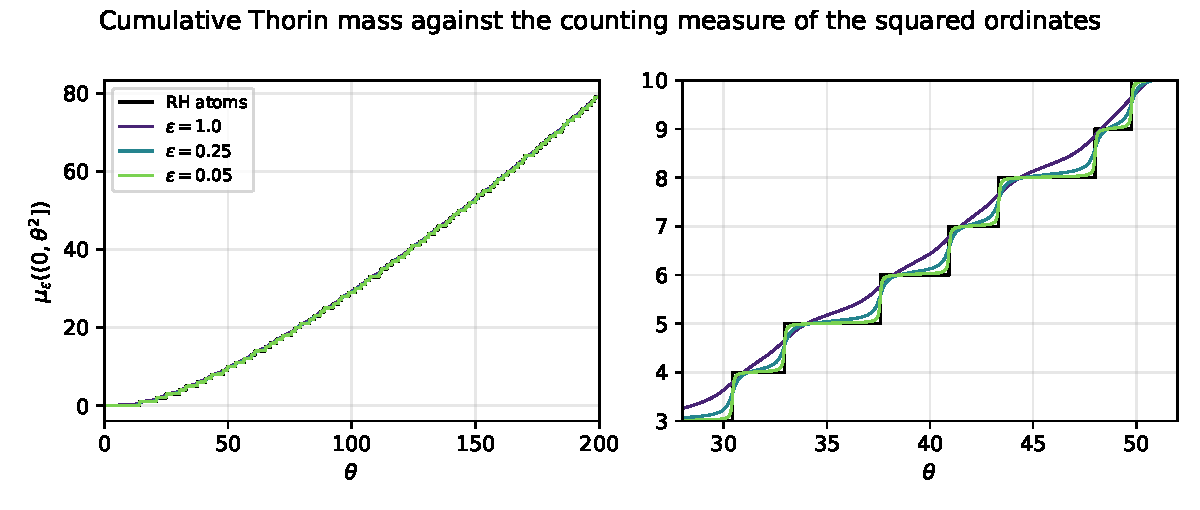
\includegraphics[width=0.95\textwidth]{fig/cumulative.pdf}
\caption{Cumulative Thorin mass $\mu_\varepsilon((0,\theta^2])=\pi^{-1}\arg\xi(\tfrac12+\varepsilon+i\theta)$ at $\varepsilon=1$, $0.25$ and $0.05$ against the counting function of $U_{\RH}$, on the whole window (left) and on $28\le\theta\le52$ (right).}
\label{fig:cumulative}
\end{figure}

Summing over cells gives a distance that resolves the individual zeros. Let $b_0=0$, $b_k=(\gamma_k+\gamma_{k+1})/2$ for $1\le k\le78$ and $b_{79}=\Theta$, and let $C_k=(b_{k-1},b_k]$. The cell masses $\mu_\varepsilon(C_k)=M_\varepsilon(b_k)-M_\varepsilon(b_{k-1})$ are differences of the argument, and the coarse grained distance
\[
d_{\rm cell}(\varepsilon)=\sum_k|\mu_\varepsilon(C_k)-1|
\]
is the total variation distance between the images of $\mu_\varepsilon$ and $U_{\RH}$ under the map sending each cell to its atom. No $b_k$ is an ordinate, so Proposition~\ref{prop:mass} applies at both ends of every cell, with $\Xi'(0)=0$ at $b_0$, and with the remainder of Remark~\ref{rem:ch7:cubic} gives $\mu_\varepsilon(C_k)-1=-(\varepsilon/\pi)\big[\Xi'/\Xi(b_k)-\Xi'/\Xi(b_{k-1})\big]+O(\varepsilon^3)$. Hence $d_{\rm cell}(\varepsilon)=\kappa_{\rm cell}\,\varepsilon+O(\varepsilon^3)$, where $\kappa_{\rm cell}=\pi^{-1}\sum_k|\Xi'/\Xi(b_k)-\Xi'/\Xi(b_{k-1})|$, the cell constant of this window, is $5.43665$, and every cell mass lies in $[0.99888,1.00126]$ at $\varepsilon=0.005$. Section~\ref{ch:spacing} reads this constant as a statistic of the irregularity of the spacings.

The $L^1$ distance $\int_0^\Theta|M_\varepsilon(\theta)-N(\theta)|\,d\theta$ between the cumulative mass and the counting function is a transport distance, and because of the Cauchy tails it behaves like $\varepsilon\log(1/\varepsilon)$: it is $1.55$ in $\theta$ and $360$ in $z$ at $\varepsilon=0.005$, and Section~\ref{sec:ch9:mass} derives the rate. The heat trace $W(t)=\int e^{-tz}U_{\RH}(dz)$ is approximated by $W_\varepsilon(t)=\int_0^\infty e^{-t\theta^2}\rho_\varepsilon(\theta)\,d\theta=\int e^{-tz}\mu_\varepsilon(dz)$. At $t=0.01$ the zeros give $W=0.1496980112538$ (Table~\ref{tab:ch2:W}), while $W_\varepsilon(0.01)=0.1504500280599$, $0.1512017825455$ and $0.1527045050533$ at $\varepsilon=0.005$, $0.01$ and $0.02$, again with error linear in $\varepsilon$.

The mass and the heat trace are smooth in $\varepsilon$ at $\varepsilon=0$, so Richardson extrapolation applies to them: the mass by Proposition~\ref{prop:mass}, and the heat trace because by Proposition~\ref{prop:struct} it is a sum over the zeros of Poisson integrals of the Gaussian $e^{-t\theta^2}$. The combination $2\mu_{0.005}(E)-\mu_{0.01}(E)$ equals $79+3.2\times10^{-8}$, against a raw defect of $2.0\times10^{-3}$. For the heat trace the error $7.5\times10^{-4}$ of $W_{0.005}(0.01)$ falls to $2.6\times10^{-7}$ after one Richardson step ($\varepsilon=0.005$ and $0.01$) and to $1.7\times10^{-10}$ after two (adding $\varepsilon=0.02$). Without extrapolation the same accuracy would need $\varepsilon\approx8\times10^{-8}$ for the mass, and $\varepsilon\approx2\times10^{-6}$ and $10^{-9}$ for the heat trace.

